\documentclass[12pt]{article} % Classe de document avec une taille de police de 12pt
\usepackage{enumitem}
\usepackage{graphicx}
\usepackage{multicol}
\usepackage[margin=1in]{geometry}
\setlength{\columnseprule}{0.4pt}
% Packages utilisés
\usepackage{geometry} % Pour modifier les marges
\usepackage{mathptmx} % Police Times New Roman
\usepackage[utf8]{inputenc} % Encodage
\usepackage[T1]{fontenc}
\usepackage{titlesec}
\usepackage{titling}
\usepackage{algorithm}
\usepackage{algpseudocode}
\usepackage{amsmath}
\usepackage{amsfonts}


% Configuration des marges
\geometry{
	a4paper,
	left=20mm,
	right=20mm,
	top=30mm,
	bottom=30mm
}


%\algnewcommand\algorithmicinput{\textbf{entrée:}}
%\algnewcommand\algorithmicoutput{\textbf{sortie:}}
\algnewcommand\algorithmicvariables{\textbf{var:}}
\algnewcommand\algorithmicstart{\textbf{début}}
\algnewcommand\Input{\item[\algorithmicinput]}
\algnewcommand\Output{\item[\algorithmicoutput]}
\algnewcommand\Variables{\item[\algorithmicvariables]}
\algnewcommand\Start{\State \algorithmicstart}
\algnewcommand\Create{\algorithmiccreate}
\algnewcommand\Size{\algorithmicsize}

\renewcommand{\algorithmicrequire}{\textbf{Entrée:}}
\renewcommand{\algorithmicensure}{\textbf{Sortie:}}

% Personnalisation de la commande \maketitle
\pretitle{\begin{center}\LARGE\bfseries}
	\posttitle{\end{center}\vskip 0.5em}
\preauthor{\begin{center}\large}
	\postauthor{\end{center}}
\predate{\begin{center}\large}
	\postdate{\end{center}\vskip 0.5em}

\title{Simulation de Bureau de Vote :\\ Conception et Implémentation en C++}
\author{AZANDOSSESSI Jaurès \\ JEAN Karl}
\date{\today}

\begin{document}
	
	\maketitle
	
	\begin{abstract}
		Ce rapport détaille la conception et l'implémentation d'une simulation informatisée d'un bureau de vote en C++. Notre objectif est de proposer un environnement de simulation réaliste et fonctionnel qui reproduise avec précision le processus électoral, de l'enregistrement des électeurs au dépouillement des votes et à la détermination du gagnant. Nous explorons les diverses étapes de développement de notre simulation, en mettant en exergue les choix de conception, les structures de données et les algorithmes utilisés pour le traitement des votes. Les fonctionnalités mises en place, les défis rencontrés et les perspectives d'amélioration sont également abordés. En définitive, notre simulation se présente comme une application concrète des principes de la programmation orientée objet et de la manipulation de données en C++, offrant un outil efficace pour l'étude et l'expérimentation des mécanismes électoraux. Ce projet enrichit non seulement nos compétences en programmation et en algorithmique, mais contribue aussi à une meilleure compréhension des dynamiques électorales.
	\end{abstract}
	
	\newpage
	

	
	\newpage
			
	\section*{Introduction}
	La simulation informatique est un outil puissant pour modéliser et analyser divers phénomènes du monde réel. Dans le domaine de la politique et de la démocratie, la simulation de bureaux de vote revêt une importance particulière. En effet, elle permet d'évaluer l'efficacité des processus électoraux, de tester différentes méthodes de vote et de prédire les résultats des élections.
	
	Dans le cadre de ce projet de programmation orientée C++, nous avons entrepris la conception et l'implémentation d'une simulation de bureau de vote. Notre objectif principal est de créer un système informatique réaliste et fonctionnel qui reproduit fidèlement le déroulement d'une élection. Cette simulation sera capable de gérer l'enregistrement des électeurs, le dépouillement des votes, et la détermination du vainqueur selon les règles du scrutin utilisé.
	
	Au cours de ce rapport, nous détaillerons les différentes étapes de développement de notre simulation, en mettant en lumière les choix de conception, les structures de données utilisées, ainsi que les algorithmes de traitement des votes. Nous discuterons également des fonctionnalités implémentées, des défis rencontrés et des perspectives d'amélioration pour ce projet.
	
	En fin de compte, cette simulation de bureau de vote constitue une application concrète des concepts de programmation orientée objet et de manipulation de données en C++. Elle représente un moyen efficace pour étudier et expérimenter avec les mécanismes électoraux, tout en renforçant nos compétences en programmation et en algorithmique.
	
	\newpage
	
\section*{Description des Classes}

\begin{itemize}[leftmargin=*,label={}]
	\item \textbf{Classe Personne}
	
	\item \textit{Description :} La classe \texttt{Personne} dans l'espace de nommage elections représente un individu participant à un processus électoral, caractérisé par son nom, son prénom, une sensibilité politique sur une échelle de 1 à 10 (de gauche à droite), et un identifiant unique généré automatiquement. 
	
	\item \textbf{Classe Electeur}
	
	\textit{Description :} La classe \texttt{Electeur}, en héritant de \texttt{Personne}, incarne un électeur au sein d'une simulation de vote. Elle est équipée d'attributs essentiels au déroulement du vote, tels que la gestion des bulletins et l'enregistrement du choix dans l'isoloir, tout en permettant le suivi du temps passé par l'électeur dans diverses zones du bureau de vote. Les méthodes intégrées facilitent l'exercice du devoir civique de l'électeur : sélection des bulletins à la table de décharge, prise de décision dans l'isoloir basée sur la probabilité et l'écart de sensibilité politique avec les candidats, et enfin, le vote. La classe offre également la possibilité d'éliminer les bulletins inutilisés à la conclusion du processus.
	
	\item \textbf{Classe TableDeDecharge} :
	
	\textit{Description :} La classe \texttt{TableDeDecharge} représente un élément crucial du processus électoral dans une simulation de vote, où elle gère l'organisation et la distribution des bulletins de vote aux électeurs. Conçue pour simuler l'espace restreint où les électeurs sélectionnent leurs bulletins, triés par candidat, elle intègre une règle stricte d'occupation singulière, assurant qu'un seul électeur à la fois puisse accéder à cet espace.
	Elle offre également des méthodes pour simuler l'entrée et la sortie des électeurs, le traitement de la file d'attente, et la gestion du temps passé par chaque électeur. En outre, elle permet de visualiser les bulletins et de gérer le flux des électeurs, faisant d'elle un pivot autour duquel s'articule l'expérience de vote dans la simulation. 
	
	\item \textbf{Classe Bulletins} :
	
	\textit{Description :} La classe \texttt{Bulletin} est conçue pour représenter de manière abstraite chaque vote au sein d'une simulation de processus électoral, incarnant le choix d'un électeur envers un candidat spécifique. Au-delà d'une simple association avec un nom de candidat, elle intègre une dimension de sensibilité politique, permettant de nuancer l'acte de vote en fonction des orientations politiques des candidats. Cette conception offre une flexibilité essentielle pour simuler avec précision divers scénarios électoraux, allant du simple dépouillement des voix à des analyses plus complexes basées sur les inclinaisons politiques. En dotant chaque bulletin d'une capacité à refléter non seulement un choix mais aussi une tendance politique, la classe devient un pivot autour duquel s'articulent les mécanismes de simulation, contribuant à une représentation plus riche et nuancée du vote. Elle est ainsi au cœur de la dynamique électorale du projet, facilitant l'exploration de différentes configurations électorales et l'évaluation de leur impact sur les résultats finaux.
	\item \textbf{Classe Elections} :
	
	\textit{Description :} La classe \texttt{Election} sert à modéliser le concept d'une élection dans une simulation ou une application liée à des processus électoraux. Elle encapsule l'essence d'une élection en associant un nom spécifique à l'événement électoral et en gérant une collection de candidats y participant. Cette gestion comprend l'enregistrement des candidats, assurant leur unicité grâce à une structure de données adaptée, et la capacité d'afficher de manière ordonnée la liste des candidats pour faciliter la consultation par les utilisateurs ou d'autres composants du système. Par cette structuration, \texttt{Election} devient un pilier pour la représentation des élections, permettant non seulement de recueillir mais aussi de diffuser les informations relatives aux options disponibles pour les électeurs. En résumant, cette classe fournit un cadre pour la mise en œuvre de la logique électorale, centralisant les données essentielles à la compréhension et à la gestion d'une élection, telles que son intitulé et les acteurs en compétition, facilitant ainsi l'interaction avec le processus électoral dans son ensemble.
	
	\item \textbf{Classe Action} :
	
	\textit{Description :} La classe \texttt{Action} incarne le concept d'une interface au sein d'un système de simulation électorale, définissant un cadre pour les interactions fondamentales des électeurs avec différents espaces électoraux tels que la table de décharge, l'isoloir, entre autres. En tant que classe abstraite, elle spécifie trois méthodes virtuelles pures, entrer, sortir, et gestionTemps, imposant ainsi aux classes dérivées la mise en œuvre de ces interactions essentielles. Cette abstraction permet d'unifier le comportement des différentes composantes du processus de vote, en garantissant que chaque espace implémente des mécanismes pour accueillir et libérer les électeurs, ainsi que pour gérer le temps passé par ces derniers dans chaque espace.
	
	\item \textbf{Classe EspaceIsoloirs} :
	
	\textit{Description :} La classe \texttt{EspaceIsoloirs} est conçue pour simuler la gestion et le fonctionnement des isoloirs au sein d'un bureau de vote durant une élection. Elle encapsule toute la logique nécessaire pour maintenir et opérer un ensemble d'isoloirs, permettant d'ajouter des isoloirs, de rechercher un isoloir libre pour un électeur, et de gérer l'entrée d'électeurs dans ces isoloirs. La classe offre des méthodes pour identifier le premier isoloir libre, reflétant ainsi une gestion efficace des ressources disponibles, et pour traiter les électeurs en attente, garantissant que chaque électeur soit dirigé vers un isoloir libre dès que possible. Elle intègre également des mécanismes pour surveiller l'état d'occupation des isoloirs et pour gérer la file d'attente d'électeurs, assurant un flux continu et ordonné au sein du bureau de vote.
	
	\item \textbf{Classe Isoloir} :
	
	\textit{Description :} La classe \texttt{Isoloir} modélise un espace individuel de vote au sein d'un bureau électoral, où les électeurs exécutent le processus de sélection de leur vote en toute confidentialité. Héritant de la classe abstraite \texttt{Action}, elle implémente les interactions essentielles d'entrée et de sortie des électeurs, ainsi que la gestion du temps passé à l'intérieur.  La méthode \texttt{choisirBulletin} encapsule la logique de sélection du vote, qui peut varier d'un choix éclairé à un vote nul basé sur une probabilité prédéterminée. \texttt{Isoloir} fournit un cadre détaillé et fonctionnel pour simuler le passage des électeurs à travers le processus de vote, depuis l'entrée jusqu'à la sélection du bulletin et la sortie, contribuant ainsi à la fidélité et à la complexité de la simulation électorale.
	
	\item \textbf{Classe TableDeVote} :
	
	\textit{Description :} La classe \texttt{TableDeVote} incarne le cœur du processus électoral dans une simulation de vote, en simulant l'espace crucial où les électeurs exécutent leur droit de vote sous la supervision du président de l'élection. Elle assure l'unicité de la présence dans cet espace via une gestion rigoureuse de l'occupation et facilite le dépôt des bulletins de vote dans l'urne ainsi que l'émargement, étape finale du processus de vote. En plus de ces opérations, la classe est dotée de fonctions pour la gestion du temps que chaque électeur passe au sein de cet espace, la vérification de la participation via une liste d'émargement et le traitement des files d'attente, garantissant une expérience de vote ordonnée et conforme aux règles établies. Un aspect fondamental de \texttt{TableDeVote} réside dans sa capacité à compiler et fournir les résultats du vote, reflétant ainsi l'issue de l'élection avec précision et intégrité. Elle joue un rôle déterminant dans la simulation, assurant non seulement le bon déroulement du vote mais aussi la fiabilité et la transparence des résultats électoraux.
	
	\item \textbf{Classe Bureau} :
	
	\textit{Description :} La classe \texttt{Bureau} encapsule le fonctionnement intégral d'un bureau de vote dans le cadre d'une simulation électorale, englobant l'enregistrement des électeurs, la gestion des candidats, et l'orchestration du processus de vote. Elle facilite l'ouverture et la fermeture de l'entrée du bureau pour réguler le flux d'électeurs, gère les interactions avec les espaces clés tels que la table de décharge, la table de vote, et les isoloirs, et assure le bon déroulement du vote jusqu'à la compilation des résultats. En intégrant des méthodes pour afficher les listes électorales, simuler l'élection, et présenter les statistiques finales, \texttt{Bureau} sert de noyau central pour la simulation, reflétant fidèlement les complexités et les dynamiques d'un véritable environnement électoral.
	
\end{itemize}	
\section*{\centering Parcours des électeurs dans notre application}

\begin{center}
	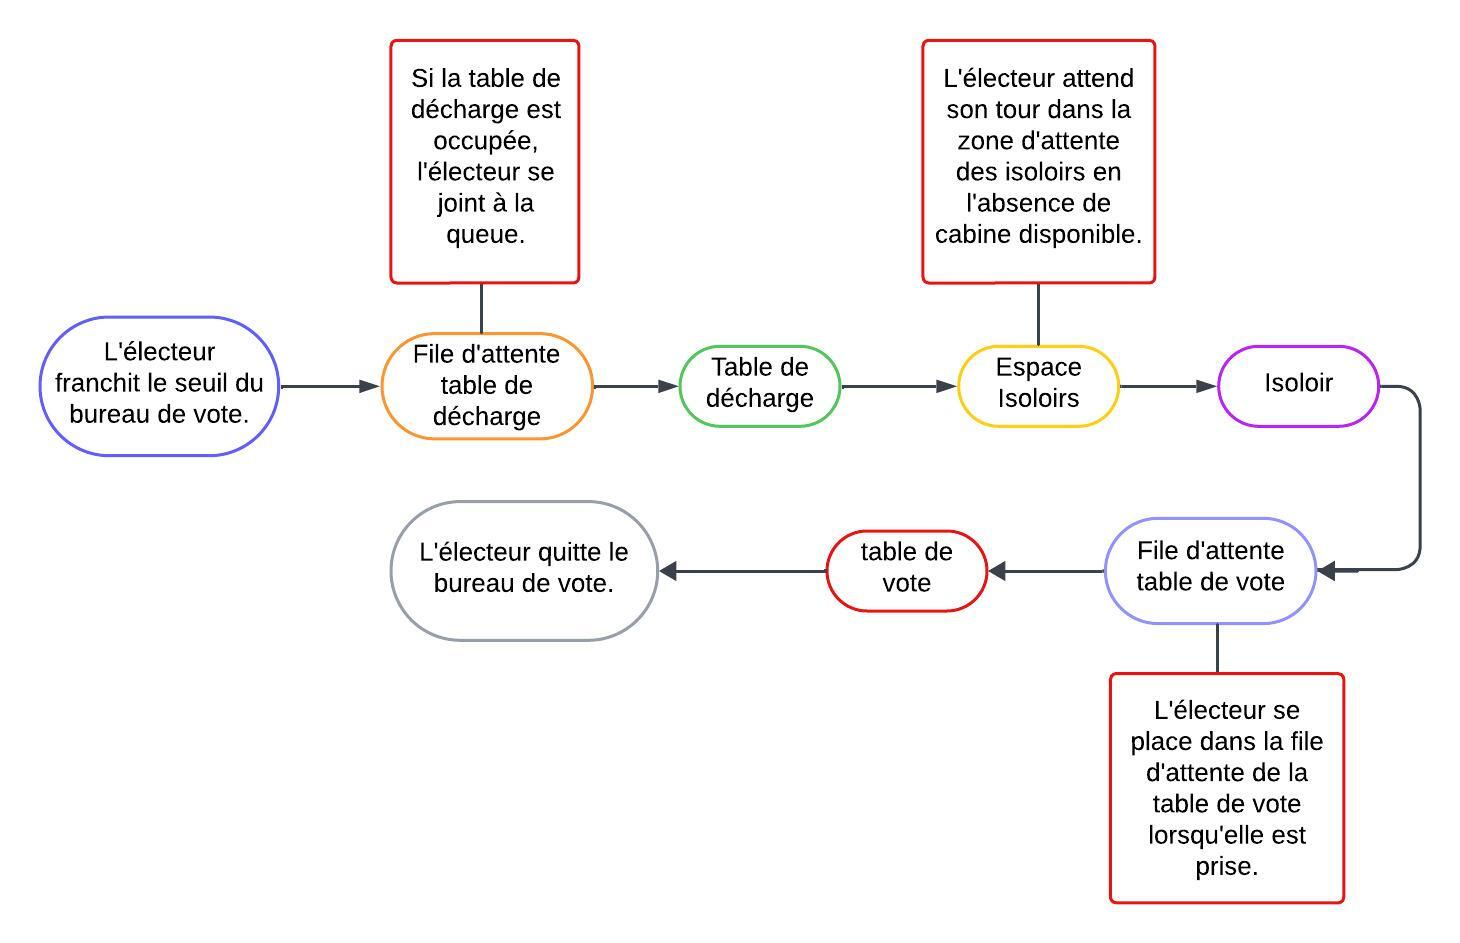
\includegraphics[width=\textwidth]{C:/Users/jaure/Documents/bureaudevote/parcours_electeur}
\end{center}

\newpage

\section*{Analyse de Complexité et Choix des Structures de Données pour les Listes Électorales}
\subsection*{Liste d'Émargement}

Pour la \textbf{liste d'émargement}, l'utilisation d'un \texttt{std::unordered\_set} s'est avérée être la solution optimale, principalement grâce à sa fondation sur une table de hachage qui facilite des opérations rapides d'insertion, de suppression, et de test d'appartenance. L'ordonnancement des éléments n'étant pas une priorité pour cette structure, le \texttt{std::unordered\_set} se montre particulièrement adapté aux besoins de la liste d'émargement. En ce qui concerne la complexité des opérations de test d'appartenance, elles se réalisent en moyenne en \textbf{O(1)}. Cependant, il est important de noter que dans des cas extrêmes, notamment en présence de nombreuses collisions de hachage, cette complexité peut se dégrader vers \textbf{O(n)}. Cette situation reste néanmoins peu fréquente, grâce à l'efficacité des mécanismes de gestion des collisions intégrés à la structure de la table de hachage.

\subsection*{Liste Électorale}

Pour la gestion de la \textbf{liste électorale}, la structure \texttt{std::set} s'est révélée être la plus appropriée. Cette décision repose sur deux principales exigences du projet : le besoin d'une liste électorale triée par ordre alphabétique et l'importance d'éviter les doublons pour maintenir l'intégrité de la liste. Le \texttt{std::set}, en tant que structure d'ensemble, réalise le tri automatiquement, facilité par l'ajout d'une fonction auxiliaire dédiée. Cette capacité à trier et à gérer de manière efficace les insertions rend le \texttt{std::set} idéal pour notre contexte, où la redondance d'éléments est inacceptable. En effet, dès qu'un élément existe déjà dans l'ensemble, toute tentative d'insertion d'un élément identique est automatiquement rejetée, assurant ainsi l'unicité des électeurs dans la liste.

Quant à la complexité des opérations de test d'appartenance, grâce à la structure interne du \texttt{std::set}, qui est basée sur un arbre binaire de recherche équilibré, cette opération est réalisée avec une complexité de \textbf{O(log n)}. Cette efficience permet de maintenir des performances élevées même à mesure que la taille de la liste s'accroît, répondant ainsi aux besoins de gestion efficace et ordonnée des électeurs inscrits dans la liste électorale.

\newpage

\section*{Ressources requises pour l'élaboration des Structures de Données Concrètes (SDC)}

Dans le cadre de l'adoption des principes d'encapsulation de la programmation orientée objet, chaque classe a été équipée des fonctions essentielles à ses responsabilités. Ainsi, diverses méthodes de la classe \textbf{Electeur} sont sollicitées par les classes Isoloir et Espace Isoloirs. Un exemple marquant est la procédure \textbf{decision}, qui permet à un électeur de finaliser son choix de candidat en sélectionnant parmi les bulletins pris sur la table de décharge. Pour une meilleure compréhension des Structures de Données Concrètes (SDC) décrites ultérieurement, nous détaillerons dans cette section toutes les fonctions mises en œuvre dans la classe \textbf{Electeur}.

\begin{flushleft}
	\begin{minipage}[t]{0.5\textwidth}
		\textbf{type} Bulletin = \textbf{Enregistrement}\\
		\hspace*{1em} \textbf{chaîne de caractères} nomCandidat;\\
		\hspace*{1em} \textbf{entier} sensibilitePolitique;\\
		\textbf{fin enregistrement}
	\end{minipage}%
	\hfill
	\begin{minipage}[t]{0.5\textwidth}
		\textbf{type} tabCapa = \textbf{Enregistrement}\\
		\hspace*{1em} \textbf{entier} capacite;\\
		\hspace*{1em} \textbf{entier} occupation;\\
		\hspace*{1em} \textbf{pointeur vers tableau de Bulletin} tab;\\ 
		\textbf{fin enregistrement}
	\end{minipage}
\end{flushleft}

\begin{flushleft}
	\textbf{type} Electeur = \textbf{Enregistrement}\\
	\hspace*{1em} \textbf{entier} duree;\\
	\hspace*{1em} \textbf{tabCapa} bulletins;\\
	\hspace*{1em} \textbf{chaîne de caractères} choix;\\
	\hspace*{1em} \textbf{booleen} estEntree;\\
	\hspace*{1em}  \textbf{booleen} estEntreeDecharge;\\
	\hspace*{1em}  \textbf{booleen} estDansEspaceIsoloir;\\
	\hspace*{1em}  \textbf{booleen} estEntreeIsoloir;\\
	\hspace*{1em}  \textbf{booleen} estEntreeTableDeVote;\\
	\hspace*{1em}  \textbf{booleen} aPrisSesBulletins;\\
	\hspace*{1em}  \textbf{booleen} aFaitSonChoix;\\
	\textbf{fin enregistrement}
\end{flushleft}

\newpage
\subsection*{Fonctions de la classe Electeur}
\begin{algorithm}
	\caption{\textbf{assignerDuree}(\underline{inout} Electeur e, \underline{in} entier temps)}
	\begin{algorithmic}[1]
		\Start
		\State e.duree $\leftarrow$ temps;
		\State Fin
	\end{algorithmic}
\end{algorithm}

\begin{algorithm}
	\caption{\textbf{validerEntreeIsoloir}(\underline{inout} Electeur e)}
	\begin{algorithmic}[1]
		\Start
		\State e.estEntreeIsoloir $\leftarrow$ true;
		\State Fin
	\end{algorithmic}
\end{algorithm}

\begin{algorithm}
	\caption{\textbf{obtenirDuree}(\underline{inout} Electeur e) $\rightarrow$ entier}
	\begin{algorithmic}[1]
		\Start
		\State retourner e.duree;
		\State Fin
	\end{algorithmic}
\end{algorithm}

\newpage

\begin{algorithm}
	\caption{\textbf{modificationDuree}(\underline{inout} Electeur e)}
	\begin{algorithmic}[1]
		\Start
		\State e.duree $\leftarrow$ e.duree - 1;
		\State Fin
	\end{algorithmic}
\end{algorithm}

\begin{algorithm}
	\caption{\textbf{validerChoixDeCandidat}(\underline{inout} Electeur e)}
	\begin{algorithmic}[1]
		\Start
		\State e.aFaitSonChoix $\leftarrow$ true;
		\State Fin
	\end{algorithmic}
\end{algorithm}

\begin{algorithm}
	\caption{\textbf{decision}(\underline{inout} Electeur e, \underline{in} reel pn, \underline{in} entier dmax)}
	\begin{algorithmic}[1]
		\State \textbf{variables}\\ \textbf{reel} probability;\\ \textbf{entier} i;\\ \textbf{chaîne de caractères} meilleurChoix;\\ \textbf{entier} meilleureDistance;\\ \textbf{chaîne de caractères} blanc;\\ \textbf{entier} distance;
		\Start
		\State probability $\leftarrow$ generer\_nombre\_alatoire(); \Comment{génère un nombre aléatoire entre 0 et 1}
		\State meilleurChoix $\leftarrow$ "";
		\State blanc $\leftarrow$ "";
		\State meilleureDistance $\leftarrow$ dmax + 1;
		\State si probability < pn alors
		\State \hspace{\algorithmicindent} e.choix $\leftarrow$ "nul";
		\State sinon
		\State \hspace{\algorithmicindent} pour i allant de 1 à e.bulletins.occupation faire
		\State \hspace{\algorithmicindent}\hspace{\algorithmicindent} si obtenirNomCandidat(mem(e.bulletins.tab)[i]) = "blanc" et est\_vide(blanc) alors
		\State \hspace{\algorithmicindent}\hspace{\algorithmicindent}\hspace{\algorithmicindent} blanc $\leftarrow$ obtenirNomCandidat(mem(e.bulletins.tab)[i]);
		\State \hspace{\algorithmicindent}\hspace{\algorithmicindent} finsi
		\State \hspace{\algorithmicindent}\hspace{\algorithmicindent} distance = valeur\_absolue(spol(e) - obtenirSensibilitePolitique(mem(e.bulletins.tab)[i]));
		\State \hspace{\algorithmicindent}\hspace{\algorithmicindent} si distance <= dmax et (est\_vide(meilleurChoix) ou distance < meilleurDistance)
		\State \hspace{\algorithmicindent}\hspace{\algorithmicindent}\hspace{\algorithmicindent} meileurChoix $\leftarrow$ obtenirNomCandidat(mem(e.bulletins.tab)[i]);
		\State \hspace{\algorithmicindent}\hspace{\algorithmicindent}\hspace{\algorithmicindent} meilleureDistance $\leftarrow$ distance;
		\State \hspace{\algorithmicindent}\hspace{\algorithmicindent} finsi 
		\State \hspace{\algorithmicindent} fin pour
		\State \hspace{\algorithmicindent} si est\_vide(meilleurChoix) alors
		\State \hspace{\algorithmicindent} \hspace{\algorithmicindent} si !est\_vide(blanc) alors
		\State \hspace{\algorithmicindent} \hspace{\algorithmicindent} \hspace{\algorithmicindent} meilleurChoix $\leftarrow$ blanc;
		\State \hspace{\algorithmicindent} \hspace{\algorithmicindent} finsi
		\State \hspace{\algorithmicindent} finsi
		\State \hspace{\algorithmicindent} si est\_vide(meilleurChoix) alors
		\State \hspace{\algorithmicindent} \hspace{\algorithmicindent} e.choix $\leftarrow$ "nul";
		\State\hspace{\algorithmicindent} sinon
		\State\hspace{\algorithmicindent}\hspace{\algorithmicindent} e.choix $\leftarrow$ meilleurChoix;
		\State\hspace{\algorithmicindent} fin sinon
		\State ecrire("   ISOLOIR");
		\State ecrire("      " + (id(e)+1) + " choisit " + e.choix)
		\State Fin
	\end{algorithmic}
\end{algorithm}

\newpage
\section*{SDA et SDC d'un isoloir}

\subsection*{SDA d'un isoloir}
Isoloir est le type d'un isoloir dans un bureau de vote muni des opérations suivantes:
\begin{itemize}
\item \textbf{creer\_isoloir}(\underline{in} reel pn, \underline{in} entier duree, \underline{in} dp, \underline{in} compteurId, \underline{out} Isoloir iso)
	\begin{description}
		\item[sortie :] $iso$ est un isoloir vide.
	\end{description}
	
	\item \textbf{entrer\_dans\_isoloir}(\underline{inout} Isoloir iso, \underline{in} Electeur* e)
	\begin{description}
		\item[pré :] $iso$ doit être vide.
		\item[rôle :] Permet de faire rentrer un électeur dans un isoloir vide.
	\end{description}
	
	\item \textbf{gestion\_temps}(\underline{inout} Isoloir iso)
	\begin{description}
		\item[pré :] $iso$ doit contenir un électeur.
		\item[rôle :] Permet de contrôler la durée d'un dans un isoloir.
	\end{description}
	\item \textbf{choisirBulletin}(\underline{inout} Isoloir iso)
	\begin{description}
		\item[pré :] $iso$ n'est pas vide.
		\item[rôle :] Permet à un électeur de faire son choix de bulletin parmi le lots de bulletins pris sur la table de décharge.
	\end{description}
	\item \textbf{sortir\_isoloir}(\underline{inout} Isoloir iso)
	\begin{description}
		\item[pré :] $iso$ n'est pas vide.
		\item[Séquence d'exécution :] L'électeur présent dans l'isoloir sort.
	\end{description}
	\item \textbf{est\_occupe}(\underline{inout} Isoloir iso)$\rightarrow$ \textbf{booléen}
	\begin{description}
		\item[sortie :] retourne vrai si l'isoloir est occupé, faux sinon.
	\end{description}
\end{itemize}

\newpage

\subsection*{SDC d'un isoloir}

\begin{flushleft}
		\textbf{type} Isoloir = \textbf{Enregistrement}\\
		\hspace*{1em} \textbf{booléen} isoloirOccupe;\\
		\hspace*{1em} \textbf{entier} idIsoloir;\\
		\hspace*{1em} \textbf{entier} distance;\\
		\hspace*{1em} \textbf{entier} dureeIsoloir\\
		\hspace*{1em} \textbf{réel} probabiliteNulle ;\\
		\hspace*{1em} \textbf{pointeur vers Electeur} electeurPresent;\\
		\textbf{fin enregistrement}
\end{flushleft}



\begin{algorithm}
	\caption{\textbf{creer\_isoloir}(\underline{in} reel pn, \underline{in} entier duree, \underline{in} dp, \underline{in} compteurId, \underline{out} Isoloir iso)}
	\begin{algorithmic}[1]
		\Start
		\State iso.isoloirOccupe $\leftarrow$ false;
		\State iso.idIsoloir $\leftarrow$ compteurId;
		\State iso.distance $\leftarrow$ dp; \Comment{\textbf{Coût} : Constant $O(1)$}
		\State iso.dureeIsoloir $\leftarrow$ duree;
		\State iso.probabiliteNulle $\leftarrow$ pn;
		\State iso.electeuurPresent $\leftarrow$ \texttt{nullptr};
		\State Fin
	\end{algorithmic}
\end{algorithm}

\begin{algorithm}
	\caption{\textbf{entrer\_dans\_isoloir}(\underline{inout} Isoloir iso, \underline{in} Electeur* e)}
	\begin{algorithmic}[1]
		\Start
		\State iso.electeurPresent $\leftarrow$ \texttt{adresse(e)};
		\State iso.isoloirOccupe $\leftarrow$ true;
		\State assignerDuree(mem(e), iso.dureeIsoloir); \Comment{\textbf{Coût} : Constant $O(1)$}
		\State validerEntreeIsoloir(e);
		\State ecrire("   ISOLOIR");
		\State ecrire("      "+id(mem(e))+1+" "+"entre");
		\State Fin
	\end{algorithmic}
	\end{algorithm}
	
	\begin{algorithm}
		\caption{\textbf{choisirBulletin}(\underline{inout} Isoloir iso)}
		\begin{algorithmic}[1]
			\Start
			\State decision(mem(iso.electeurPrsent), iso.probabiliteNulle, iso.distance); \Comment{\textbf{Coût} : Linéaire $O(N)$}
			\State Fin
		\end{algorithmic}
	\end{algorithm}
	
La procédure $decision$ examine séquentiellement la liste des bulletins que l'électeur a collectés à la table de décharge. Elle sélectionne le bulletin correspondant au candidat de préférence, basé sur l'alignement de la sensibilité politique de l'électeur avec celle indiquée sur le bulletin. Le nombre total de bulletins examinés au cours de cette procédure est désigné par \( N \).
	
\newpage

\begin{algorithm}
	\caption{\textbf{sortir\_isoloir}(\underline{inout} Isoloir iso)}
	\begin{algorithmic}[1]
		\Start
		\State iso.isoloirOccupe $\leftarrow$ false;
		\State ecrire(" "+id(mem(iso.electeurPresent))+1+" "+"sort"); \Comment{\textbf{Coût} : Constant $O(1)$}
		\State validerChoixDeCandidat(mem(iso.electeurPresent));
		\State iso.electeurPresent $\leftarrow$ nullptr;
		\State Fin
		
	\end{algorithmic}
\end{algorithm}
\begin{algorithm}
	\caption{\textbf{gestion\_temps}(\underline{inout} Isoloir iso)}
	\begin{algorithmic}[1]
		\Start
		\State si iso.electeurPresent $\neq$ \texttt{nullptr} alors
		\State \hspace{\algorithmicindent} si obtenirDuree(mem(iso.electeurPresent)) $>$ 0 alors
		\State \hspace{\algorithmicindent}\hspace{\algorithmicindent}  modificationDuree(mem(iso.electeurPresent));
		\State \hspace{\algorithmicindent} fin si \Comment{\textbf{Coût} : $\Omega(1)$ $\cap$ $O(N)$}
		\State \hspace{\algorithmicindent} si obtenirDuree(mem(iso.electeurPresent)) $=$ 0 alors
		\State \hspace{\algorithmicindent}\hspace{\algorithmicindent} choisirBulletin(iso.electeurPresent);
		\State \hspace{\algorithmicindent}\hspace{\algorithmicindent} sortir\_isoloir(iso);
		\State \hspace{\algorithmicindent} fin si
		\State fin si
		\State Fin
	\end{algorithmic}
\end{algorithm}

La méthode `$gestion\_temps$` exécute des opérations de coût constant (représenté par $\Omega(1)$) quand la durée restante de l'électeur n'est pas épuisée, ce qui constitue le meilleur cas. Néanmoins, dès que le compteur de temps de l'électeur atteint zéro, à chaque itération, cette méthode invoque la procédure `$decision$`, dont le coût est linéaire, $O(N)$. Cette situation représente donc le pire des cas pour la performance de `$gestion\_temps$`.
\begin{algorithm}
	\caption{\textbf{est\_occupe}(\underline{inout} Isoloir iso)$\rightarrow$ booléen}
	\begin{algorithmic}[1]
		\Start
		\State Retourner iso.isoloirOccupe; \Comment{\textbf{Coût} : Constant $O(1)$}
		\State Fin
	\end{algorithmic}
\end{algorithm}

\newpage

\section*{SDA et SDC d'un espace d'isoloirs}
\subsection*{SDA d'un espace d'isoloirs}
EspaceIsoloirs est le type représentant un espace d'isoloirs dans un bureau de vote muni des opérations suivantes:
\begin{itemize}
	\item \textbf{creer\_espace}(\underline{in} reel pn, \underline{in} entier nombresIsoloirs, \underline{in} entier duree, \underline{in} entier dp, \underline{out} EspaceIsoloirs esp);
	\begin{description}
		\item[sortie :] $esp$ est un espace d'isoloir vide.
	\end{description}
	\item \textbf{rechercheIsoloirLibre}(\underline{inout} EspaceIsoloirs esp) $\rightarrow$ \textbf{entier}
	\begin{description}
		\item[rôle :] renvoie l'indice du premier isoloir libre.
	\end{description}
	\item \textbf{etatIsoloir}(\underline{inout} EspaceIsoloirs esp) $\rightarrow$ booleen
	\begin{description}
		\item[rôle :] retourne vrai si il y a un isoloir occupé et faux sinon.
	\end{description}
	\item \textbf{traiterFileAttente}(\underline{inout} EspaceIsoloirs esp)
	\begin{description}
		\item[rôle :] Fais passer le premier électeur de la file d'attente dans le premier isoloir libre.
	\end{description}
	\item \textbf{obtenirTailleFile}(\underline{inout} EspaceIsoloirs esp) $\rightarrow$ \textbf{entier}
		\begin{description}
		\item[rôle :] renvoie la taille de l'espace d'isoloirs c'est-à-dire le nombre d'isoloirs dans l'espace.
	\end{description}
	\item \textbf{gestionDuree}(\underline{inout} EspaceIsoloirs esp)
		\begin{description}
		\item[rôle :] contrôle le temps d'un électeur dans un isoloir occupé de l'espace.
	\end{description}
	\item \textbf{entrerIsoloirLibre}(\underline{in} Electeur* e)
	\begin{description}
		\item[rôle :] Fais rentrer l'électeur dans un isoloir libre si la file d'attente est vide sinon le fait rentrer dans la file.
	\end{description}
\end{itemize}
\newpage

\subsection*{SDC d'un espace d'isoloirs}

\begin{flushleft}
	\begin{minipage}[t]{0.5\textwidth}
	\textbf{type} Maillon = \textbf{Enregistrement}\\
	\hspace*{1em} \textbf{Electeur*} e;\\
	\hspace*{1em} \textbf{pointeur vers Maillon} suiv;\\ 
	\textbf{fin enregistrement}
	\end{minipage}%
	\hfill
	\begin{minipage}[t]{0.5\textwidth}
		\textbf{type} fileElecteur = \textbf{Enregistrement}\\
		\hspace*{1em} \textbf{entier} nombresElecteurs;\\
		\hspace*{1em} \textbf{pointeur vers Maillon} premier;\\
		\hspace*{1em} \textbf{pointeur vers Maillon} dernier;\\ 
		\textbf{fin enregistrement}
	\end{minipage}
\end{flushleft}

\begin{flushleft}
	\begin{minipage}[t]{0.5\textwidth}
		\textbf{type} tabCapaEspace = \textbf{Enregistrement}\\
		\hspace*{1em} \textbf{entier} capacite;\\
		\hspace*{1em} \textbf{entier} occupation;\\
		\hspace*{1em} \textbf{pointeur vers tableau de Isoloir} tableau;\\ 
		\textbf{fin enregistrement}
	\end{minipage}%
	\hfill
	\begin{minipage}[t]{0.5\textwidth}
		\textbf{type} EspaceIsoloirs = \textbf{Enregistrement}\\
		\hspace*{1em} \textbf{tabCapaEspace} espaceIsoloirs;\\
		\hspace*{1em} \textbf{fileElecteur} fileAttenteIsoloir;\\
		\hspace*{1em} \textbf{file d'entier} isoloirsVides;\\
		\hspace*{1em} \textbf{entier} isoloirsOccupe;\\ 
		\textbf{fin enregistrement}
	\end{minipage}
\end{flushleft}

\begin{algorithm}
	\caption{\textbf{creer\_espace}(\underline{in} reel pn, \underline{in} entier nombresIsoloirs, \underline{in} entier duree, \underline{in} entier dp, \underline{out} EspaceIsoloirs esp)}
	\begin{algorithmic}[1]
		\State \textbf{variables}\\ \textbf{entier} i,\\ \textbf{Isoloir} iso;
		\Start
		\State esp.isoloirsOccupe $\leftarrow$ 0;
		\State esp.espaceIsoloirs.capacite $\leftarrow$ nombresIsoloirs;
		\State esp.espaceIsoloirs.occupation $\leftarrow$ 0;
		\State esp.espaceIsoloirs.tableau $\leftarrow$ allocation de tableau de esp.espaceIsoloirs.capacite d'Isoloir;  
		\State creer\_file(esp.fileAttenteIsoloir);
		\State creer\_file(esp.isoloirVides);  \Comment{\textbf{Coût} : Linéaire $O(N)$}
		\State pour i allant de 1 à nombresIsoloirs faire 
		\State \hspace{\algorithmicindent}  creer\_isoloir(pn, duree, dp, 200, iso);
		\State \hspace{\algorithmicindent} mem(esp.espaceIsoloirs.tableau)[i] $\leftarrow$ iso;
		\State  \hspace{\algorithmicindent} esp.espaceIsoloirs.occupation $\leftarrow$ ++;
		\State  \hspace{\algorithmicindent} enfiler(esp.isoloirVides, i);
		\State  fin pour;
		\State Fin
		
	\end{algorithmic}
\end{algorithm}

La procédure `$creer\_espace$` est conçue pour initialiser un nouvel espace d'isoloirs. Elle utilise une boucle qui itère de 1 jusqu'au nombre total d'isoloirs prévu, ce qui induit une complexité linéaire, \( O(N) \), où \( N \) représente le nombre d'isoloirs. Grâce à l'utilisation d'un tableau dynamique, aucun agrandissement ultérieur n'est nécessaire, car l'espace est configuré dès le début avec le nombre exact d'isoloirs requis. Cette approche prévient les coûts additionnels liés à un redimensionnement potentiel durant l'utilisation de l'espace isoloir.

\begin{algorithm}
	\caption{\textbf{rechercheIsoloirLibre}(\underline{inout} EspaceIsoloirs esp) $\rightarrow$ \textbf{entier}}
	\begin{algorithmic}[1]
		\State \textbf{variables}\\ \textbf{entier} indice;
		\Start
		\State si !est\_vide(esp.isoloirsVides) alors
		\State  \hspace{\algorithmicindent} indice $\leftarrow$ premier(esp.isoloirsVides); \Comment{\textbf{Coût} : Constant $O(1)$}
		\State  \hspace{\algorithmicindent} defiler(esp.isoloirsVides);
		\State  \hspace{\algorithmicindent} retourner indice;
		\State finsi ;
		\State retourner -1;
		\State Fin
	\end{algorithmic}
\end{algorithm}
\newpage

\begin{algorithm}
	\caption{\textbf{etatIsoloir}(\underline{inout} EspaceIsoloirs esp) $\rightarrow$ booleen}
	\begin{algorithmic}[1]
		\Start
		\State retourner esp.isoloirsOccupe > 0; \Comment{\textbf{Coût} : Constant $O(1)$}
		\State Fin
	\end{algorithmic}
\end{algorithm}

\begin{algorithm}
	\caption{\textbf{traiterFileAttente}(\underline{inout} EspaceIsoloirs esp)}
	\begin{algorithmic}[1]
		\State \textbf{variables}\\ \textbf{entier} indice;\\\textbf{Electeur*} prochain;
		\Start
		\State tant que !est\_vide(esp.fileAttenteIsoloir) \&\& esp.isoloirsOccupe < esp.espaceIsoloirs.occupation faire
		\State  \hspace{\algorithmicindent} indice $\leftarrow$ rechercheIsoloirLibre(esp);
		\State  \hspace{\algorithmicindent} si indice $\neq$ -1 alors \Comment{\textbf{Coût} : Linéaire $O(N)$}
		\State  \hspace{\algorithmicindent}  \hspace{\algorithmicindent} prochain $\leftarrow$ premier(esp.fileAttenteIsoloir);
		\State  \hspace{\algorithmicindent} \hspace{\algorithmicindent} defiler(esp.fileAttenteIsoloir);
		\State  \hspace{\algorithmicindent} \hspace{\algorithmicindent} entrer\_dans\_isoloir(mem(esp.espaceIsoloirs.tableau)[indice], mem(prochain));
		 \State  \hspace{\algorithmicindent} \hspace{\algorithmicindent} esp.isoloirsOccupe ++;
		 \State  \hspace{\algorithmicindent} \hspace{\algorithmicindent} finsi;
		 \State  \hspace{\algorithmicindent} fin tant que;
		\State Fin
	\end{algorithmic}
\end{algorithm}

la procédure `$traiterFileAttente$` parcourt la file d'attente et essaie de placer les électeurs dans les isoloirs libres jusqu'à ce que la file soit vide ou qu'il n'y ait plus d'isoloirs libres. Cela pourrait potentiellement impliquer de parcourir toute la file d'attente et tous les isoloirs, en fonction de leur état d'occupation.

\begin{algorithm}
	\caption{\textbf{obtenirTailleFile}(\underline{inout} EspaceIsoloirs esp) $\rightarrow$ \textbf{entier}}
	\begin{algorithmic}[1]
		\Start
		\State retourner esp.fileAttenteIsoloir.nombresElecteurs; \Comment{\textbf{Coût} : Constant $O(1)$}
		\State Fin
	\end{algorithmic}
\end{algorithm}

\newpage

\begin{algorithm}
	\caption{\textbf{gestionDuree}(\underline{inout} EspaceIsoloirs esp)}
	\begin{algorithmic}[1]
		\State \textbf{variables}\\ \textbf{entier} i;
		\Start
		\State pour i allant de 1 à esp.espaceIsoloirs.occupation faire
		\State  \hspace{\algorithmicindent} si est\_occupe(mem(esp.espaceIsoloirs.tab)[i]) alors
		\State  \hspace{\algorithmicindent} \hspace{\algorithmicindent} gestion\_temps(mem(esp.espaceIsoloirs.tab)[i]); \Comment{\textbf{Coût} : Linéaire $O(N)$}
		\State  \hspace{\algorithmicindent} \hspace{\algorithmicindent} \hspace{\algorithmicindent} si !est\_occupe(mem(esp.espaceIsoloirs.tab)[i] alors
		\State  \hspace{\algorithmicindent} \hspace{\algorithmicindent} \hspace{\algorithmicindent} \hspace{\algorithmicindent} enfiler(esp.isoloirsVides, i);
		\State  \hspace{\algorithmicindent} \hspace{\algorithmicindent} \hspace{\algorithmicindent} \hspace{\algorithmicindent} esp.isoloirsOccupe - -;
		\State  \hspace{\algorithmicindent} \hspace{\algorithmicindent} \hspace{\algorithmicindent} finsi
		\State  \hspace{\algorithmicindent} finsi
		\State fin pour
		\State Fin
	\end{algorithmic}
\end{algorithm}

Cette méthode parcourt tous les isoloirs pour mettre à jour leur état basé sur le temps restant. Chaque isoloir gère son temps, et en fonction de leur état (occupé ou non), ils peuvent être libérés, ce qui requiert une mise à jour de la liste des isoloirs libres. La complexité est linéaire en fonction du nombre d'isoloirs.

\begin{algorithm}
	\caption{\textbf{entrerIsoloirLibre}(\underline{in} Electeur* e)}
	\begin{algorithmic}[1]
		\State \textbf{variables}\\ \textbf{entier} indice;
		\Start
		\State validerPresenceEspaceIsoloir(mem(e)); \Comment{\textbf{Coût} : $\Omega(1)$ $\cap$ $O(N)$}
		\State indice $\leftarrow$ rechercheIsoloirLibre(esp);
		\State si indice $\neq$ -1 alors  
		\State  \hspace{\algorithmicindent} entrer\_dans\_isoloir(mem(esp.espaceIsoloirs.tableau)[indice], mem(e));
		\State \hspace{\algorithmicindent} esp.isoloirsOccupe ++;
		\State sinon
		\State \hspace{\algorithmicindent} enfiler(esp.fileAttenteIsoloir, mem(e));
		\State fin sinon
		\State traiterFileAttente(esp);
		\State Fin
	\end{algorithmic}
\end{algorithm}
La procédure `$entrerIsoloirLibre$` tente d'abord de placer un électeur dans un isoloir libre via la fonction `$rechercheIsoloirLibre$`, qui fonctionne à coût constant. Si aucun isoloir n'est libre, l'électeur est ajouté à la file d'attente, également à coût constant. Ensuite, `$traiterFileAttente$` est appelée pour faire avancer les électeurs dans la file vers les isoloirs libres. Si tous les isoloirs sont occupés ou la file est vide, cette opération est rapide et à coût constant. Toutefois, si des isoloirs se libèrent et que la file contient des électeurs, le coût peut devenir linéaire.

\newpage

\section*{Trace d'exécution}	
	\begin{multicols}{3}
		{\footnotesize
			\noindent
			ELECTION 'Euro 2024'\\
			\hspace*{6mm} Candidat n°0 : X nel 5\\
			\hspace*{6mm} Candidat n°1 : Y rik 2\\
			\hspace*{6mm} Candidat n°2 : Z pat 8\\
			
			\noindent BUREAU n°310\\
			LISTE ELECTORALE\\
			\hspace*{5mm} A bic (0)\\
			\hspace*{5mm} B gad (1)\\
			\hspace*{5mm} C ann (2)\\
			\hspace*{5mm} D pol (3)\\
			\hspace*{5mm} E lam (4)\\
			\hspace*{5mm} F bul (5)\\
			\hspace*{5mm} G yap (6)\\
			\hspace*{5mm} X nel (7)\\
			\hspace*{5mm} Y rik (8)\\
			\hspace*{5mm} Z pat (9)\\
			
			\noindent PREPARATION DECHARGE\\
			\hspace*{5mm} X nel : 10 bulletins\\
			\hspace*{5mm} Y rik : 10 bulletins\\
			\hspace*{5mm} Z pat : 10 bulletins\\
			
			\noindent OUVERTURE BUREAU n°310\\
			TMAX = 20\\
			
			\noindent T = 1\\
			T = 2\\
			T = 3\\
			\hspace*{5mm} ENTREE\\
			\hspace*{12mm} 4 entre\\
			\hspace*{5mm} DECHARGE\\
			\hspace*{12mm} 4 entre\\
			T = 4\\
			\hspace*{5mm} ENTREE\\
			\hspace*{12mm} 8 entre\\
			T = 5\\
			\hspace*{5mm} DECHARGE\\
			\hspace*{12mm} 4 prend Y rik\\
			\hspace*{12mm} 4 prend Z pat\\
			\hspace*{12mm} 4 prend X nel\\
			\hspace*{5mm} ENTREE\\
			\hspace*{12mm} 3 entre\\
			T = 6\\
			\hspace*{5mm} DECHARGE\\
			\hspace*{12mm} 4 sort\\
			\hspace*{5mm} ISOLOIR\\
			\hspace*{12mm} 4 entre\\
			T = 7\\
			\hspace*{5mm} DECHARGE\\
			\hspace*{12mm} 8 entre\\
			\hspace*{5mm} ENTREE\\
			\hspace*{12mm} 2 entre\\
			T = 8\\
			T = 9\\
			\hspace*{5mm} DECHARGE\\
			\hspace*{12mm} 8 prend Z pat\\
			\hspace*{12mm} 8 prend Y rik\\
			T = 10\\
			\hspace*{5mm} DECHARGE\\
			\hspace*{12mm} 8 sort\\
			\hspace*{5mm} ISOLOIR\\
			\hspace*{12mm} 8 entre\\
			T = 11\\
			\hspace*{5mm} DECHARGE\\
			\hspace*{12mm} 3 entre\\
			\hspace*{5mm} ENTREE\\
			\hspace*{12mm} 1 entre\\
			T = 12\\
			\hspace*{5mm} ISOLOIR\\
			\hspace*{12mm} 4 choisit Y rik\\
			\hspace*{12mm} 4 sort\\
			\hspace*{5mm} VOTE\\
			\hspace*{12mm} 4 entre\\
			T = 13\\
			\hspace*{5mm} DECHARGE\\
			\hspace*{12mm} 3 prend Y rik\\
			T = 14\\
			\hspace*{5mm} DECHARGE\\
			\hspace*{12mm} 3 sort\\
			\hspace*{5mm} VOTE\\
			\hspace*{12mm} 4 vote\\
			\hspace*{5mm} ISOLOIR\\
			\hspace*{12mm} 3 entre\\
			T = 15\\
			\hspace*{5mm} DECHARGE\\
			\hspace*{12mm} 2 entre\\
			\hspace*{5mm} ENTREE\\
			\hspace*{12mm} 6 entre\\
			T = 16\\
			\hspace*{5mm} ISOLOIR\\
			\hspace*{12mm} 8 choisit Z pat\\
			\hspace*{12mm} 8 sort\\
			T = 17\\
			\hspace*{5mm} DECHARGE\\
			\hspace*{12mm} 2 prend X nel\\
			\hspace*{12mm} 2 prend Z pat\\
			\hspace*{5mm} VOTE\\
			\hspace*{12mm} 4 sort\\
			\hspace*{5mm} SORTIE\\
			\hspace*{12mm} 4 sort\\
			T = 18\\
			\hspace*{5mm} DECHARGE\\
			\hspace*{12mm} 2 sort\\
			\hspace*{5mm} VOTE\\
			\hspace*{12mm} 8 entre\\
			\hspace*{5mm} ISOLOIR\\
			\hspace*{12mm} 2 entre\\
			T = 19\\
			\hspace*{5mm} DECHARGE\\
			\hspace*{12mm} 1 entre\\
			\hspace*{5mm} ENTREE\\
			\hspace*{12mm} 5 entre\\
			
			\noindent FERMETURE ENTREE\\
			
			\noindent T = 20\\
			\hspace*{5mm} ISOLOIR\\
			\hspace*{12mm} 3 choisit Y rik\\
			\hspace*{12mm} 3 sort\\
			\hspace*{5mm} VOTE\\
			\hspace*{12mm} 8 vote\\
			T = 21\\
			\hspace*{5mm} DECHARGE\\
			\hspace*{12mm} 1 prend X nel\\
			\hspace*{12mm} 1 prend Y rik\\
			T = 22\\
			\hspace*{5mm} DECHARGE\\
			\hspace*{12mm} 1 sort\\
			\hspace*{5mm} ISOLOIR\\
			\hspace*{12mm} 1 entre\\
			T = 23\\
			\hspace*{5mm} DECHARGE\\
			\hspace*{12mm} 6 entre\\
			\hspace*{5mm} VOTE\\
			\hspace*{12mm} 8 sort\\
			\hspace*{5mm} SORTIE\\
			\hspace*{12mm} 8 sort\\
			T = 24\\
			\hspace*{5mm} ISOLOIR\\
			\hspace*{12mm} 2 choisit Z pat\\
			\hspace*{12mm} 2 sort\\
			\hspace*{5mm} VOTE\\
			\hspace*{12mm} 3 entre\\
			T = 25\\
			\hspace*{5mm} DECHARGE\\
			\hspace*{12mm} 6 prend Z pat\\
			\hspace*{12mm} 6 prend X nel\\
			T = 26\\
			\hspace*{5mm} DECHARGE\\
			\hspace*{12mm} 6 sort\\
			\hspace*{5mm} VOTE\\
			\hspace*{12mm} 3 vote\\
			\hspace*{5mm} ISOLOIR\\
			\hspace*{12mm} 6 entre\\
			T = 27\\
			\hspace*{5mm} DECHARGE\\
			\hspace*{12mm} 5 entre\\
			T = 28\\
			\hspace*{5mm} ISOLOIR\\
			\hspace*{12mm} 1 choisit X nel\\
			\hspace*{12mm} 1 sort\\
			T = 29\\
			\hspace*{5mm} DECHARGE\\
			\hspace*{12mm} 5 prend X nel\\
			\hspace*{12mm} 5 prend Y rik\\
			\hspace*{5mm} VOTE\\
			\hspace*{12mm} 3 sort\\
			\hspace*{5mm} SORTIE\\
			\hspace*{12mm} 3 sort\\
			T = 30\\
			\hspace*{5mm} DECHARGE\\
			\hspace*{12mm} 5 sort\\
			\hspace*{5mm} VOTE\\
			\hspace*{12mm} 2 entre\\
			\hspace*{5mm} ISOLOIR\\
			\hspace*{12mm} 5 entre\\
			T = 31\\
			T = 32\\
			\hspace*{5mm} ISOLOIR\\
			\hspace*{12mm} 6 choisit Z pat\\
			\hspace*{12mm} 6 sort\\
			\hspace*{5mm} VOTE\\
			\hspace*{12mm} 2 vote\\
			T = 33\\
			T = 34\\
			T = 35\\
			\hspace*{5mm} VOTE\\
			\hspace*{12mm} 2 sort\\
			\hspace*{5mm} SORTIE\\
			\hspace*{12mm} 2 sort\\
			T = 36\\
			\hspace*{5mm} ISOLOIR\\
			\hspace*{12mm} 5 choisit Y rik\\
			\hspace*{12mm} 5 sort\\
			\hspace*{5mm} DECHARGE\\
			\hspace*{5mm} ISOLOIR\\
			\hspace*{5mm} VOTE\\
			\hspace*{12mm} 1 entre\\
			T = 37\\
			T = 38\\
			\hspace*{5mm} VOTE\\
			\hspace*{12mm} 1 vote\\
			T = 39\\
			T = 40\\
			T = 41\\
			\hspace*{5mm} VOTE\\
			\hspace*{12mm} 1 sort\\
			\hspace*{5mm} SORTIE\\
			\hspace*{12mm} 1 sort\\
			T = 42\\
			\hspace*{5mm} VOTE\\
			\hspace*{12mm} 6 entre\\
			T = 43\\
			T = 44\\
			\hspace*{5mm} VOTE\\
			\hspace*{12mm} 6 vote\\
			T = 45\\
			T = 46\\
			T = 47\\
			\hspace*{5mm} VOTE\\
			\hspace*{12mm} 6 sort\\
			\hspace*{5mm} SORTIE\\
			\hspace*{12mm} 6 sort\\
			T = 48\\
			\hspace*{5mm} VOTE\\
			\hspace*{12mm} 5 entre\\
			T = 49\\
			T = 50\\
			\hspace*{5mm} VOTE\\
			\hspace*{12mm} 5 vote\\
			T = 51\\
			T = 52\\
			T = 53\\
			\hspace*{5mm} VOTE\\
			\hspace*{12mm} 5 sort\\
			\hspace*{5mm} SORTIE\\
			\hspace*{12mm} 5 sort\\
			
			\noindent FERMETURE BUREAU n°310\\
			
			\noindent Bureau n°310 : RESULTATS Euro 2024 \\
			\hspace*{6mm} PRESIDENT : C ann \\
			\hspace*{6mm} nb electeurs : 10 \\
			\hspace*{6mm} nb votes : 7 \\
			\hspace*{6mm} participation : 70\% \\
			\hspace*{6mm} abstention : 30\% \\
			\hspace*{6mm} nul : 0 (0\%) \\
			\hspace*{6mm} blanc : 0 (0\%) \\
			\hspace*{6mm} Z pat : 3 (43\%) \\
			\hspace*{6mm} Y rik : 3 (43\%) \\
			\hspace*{6mm} X nel : 1 (14\%) \\
	}
	\end{multicols}
	
	\newpage
	
	\section*{Bilan du Projet}
	\subsection*{Complétude du projet}
	Dans ce projet, nous avons rigoureusement implémenté toutes les étapes essentielles du processus de vote, couvrant l'entrée dans le bureau de vote, la sélection des bulletins à la table de décharge, la prise de décision dans l'isoloir, et la formalisation finale du vote à la table de vote avec émargement. Chaque méthode a été optimisée pour minimiser les coûts d'exécution tout en maximisant la performance.
	
	Sur le plan de la programmation orientée objet, nous avons strictement respecté ses principes fondamentaux, tels que l'encapsulation, qui nous a permis de protéger l'état interne des objets et d'assurer une interface claire pour leur manipulation. En outre, l'héritage a été utilisé pour hiérarchiser et réutiliser le code efficacement, tandis que le polymorphisme a facilité l'extension et la modification des fonctionnalités sans compromettre l'architecture existante.
	
	Nous avons également intégré des tests unitaires pour chaque composant, assurant que chaque fonctionnalité répond aux exigences prévues et fonctionne correctement dans divers scénarios. Cela a été crucial pour maintenir la robustesse du système et pour simplifier les phases de débogage et de maintenance. En faisant le bilan, nous avons constaté que tous les objectifs fixés pour ce projet ont été atteints.
	
	\subsection*{Correction du projet}
	Au cours de la réalisation de ce projet, nous avons rencontré plusieurs défis, notamment des erreurs liées à la copie d'objets. Initialement, dans notre application, nous avons eu des problèmes avec la copie des objets Electeur. Cela entraînait des situations où les modifications apportées ne se répercutaient pas sur les objets concernés, ce qui rendait les mises à jour incohérentes.
	
	Ce problème s'est avéré difficile à identifier. Nous avons donc fait appel au débogueur C++ GDB, qui s'est révélé indispensable pour comprendre l'erreur. Suite à cette analyse, nous avons modifié notre approche en passant directement des pointeurs vers l'objet Electeur dans la liste électorale. Cette solution non seulement simplifiait le code, mais garantissait également la cohérence des données à travers l'application.
	
	Cette expérience a souligné l'importance de choisir judicieusement entre la copie d'objets et l'utilisation de références ou de pointeurs, surtout dans un contexte où la cohérence et l'intégrité des données sont cruciales.
	
	\subsection*{Améliorations Futures}

	Pour enrichir et structurer notre section sur les améliorations futures, nous envisageons plusieurs extensions significatives pour notre simulation de bureau de vote, afin d'accroître sa fonctionnalité et sa pertinence.
	
	\subsubsection*{Multi-bureau de vote}
	Actuellement, notre simulation se concentre sur un seul bureau de vote. Nous prévoyons d'élargir ce cadre pour inclure plusieurs bureaux de vote. Cela permettrait l'enregistrement des électeurs dans des bureaux spécifiques, basé sur des critères géographiques ou démographiques déterminés, offrant ainsi une simulation plus représentative des élections nationales ou régionales.
	
	\subsubsection*{Processus électoral complet}
	Nous souhaitons développer un processus électoral plus complet en intégrant des phases telles que les campagnes électorales, la préparation des listes électorales, et la publication des résultats. Cela enrichirait l'expérience utilisateur en fournissant un aperçu complet du cycle électoral.
	
	\subsubsection*{Amélioration de la gestion des données}
	Pour gérer efficacement l'augmentation de la complexité due à l'ajout de multiples bureaux de vote, une refonte de notre système de gestion des données sera nécessaire. Cela comprendra l'optimisation des structures de données pour un accès plus rapide et la sécurisation des informations sensibles des électeurs.
	
	\subsubsection*{Interface utilisateur interactive}
	Pour rendre notre simulation plus accessible et engageante, le développement d'une interface utilisateur graphique interactive est prévu. Cela permettrait aux utilisateurs de visualiser en temps réel les différentes étapes du processus électoral et d'interagir directement avec le système pour modifier les paramètres ou suivre des scénarios spécifiques.
	
	\subsubsection*{Analyse statistique des résultats}
	En plus de simuler le processus de vote, nous aimerions fournir des outils d'analyse statistique pour évaluer les résultats des élections, permettant aux utilisateurs de générer des rapports détaillés sur les tendances de vote, la participation, et d'autres métriques pertinentes.
	
	Ces améliorations visent non seulement à étendre les fonctionnalités de notre projet mais aussi à en faire un outil pédagogique et de recherche plus robuste pour les études en sciences politiques et en administration publique.
	
	\subsection*{Evaluation Critique}
	Notre application répond aux exigences initiales et satisfait les attentes des utilisateurs grâce aux implémentations réalisées. Un soin particulier a été apporté à la lisibilité du code, avec des noms de variables et de fonctions explicites et un commentaire exhaustif de chaque segment de code.
	
	En matière de conformité aux normes de la programmation orientée objet, nous avons intégré des éléments clés tels que le polymorphisme, l'héritage et l'encapsulation. Ces pratiques ont renforcé la structure et la robustesse de notre projet.
	
	Au cours de ce projet, nous avons acquis de nombreuses connaissances, notamment dans l'utilisation des bibliothèques C++ standard telles que \texttt{std::vector}, \texttt{std::stack}, et \texttt{std::map}. Les débuts étaient difficiles, principalement à cause de la nécessité de comprendre comment accéder et utiliser ces bibliothèques. Toutefois, ce travail assidu nous a permis de bâtir une solide compréhension des fondements de la programmation orientée objet en C++.
	
	Nous ne maîtrisons peut-être pas encore parfaitement toutes les subtilités, mais nous avons établi une base solide qui nous permettra de mener à bien des projets futurs de manière plus efficace et plus rapide.
	
	\newpage
	
	\section*{Conclusion}
	Ce projet de simulation d'un bureau de vote en C++ a été une entreprise enrichissante et formatrice qui a mis en évidence la puissance et la flexibilité de la programmation orientée objet. En adoptant une approche méthodique et structurée, nous avons réussi à concevoir et à implémenter une simulation qui non seulement répond aux exigences techniques spécifiques, mais offre également une plateforme dynamique pour comprendre les processus électoraux.
	
	Nous avons traversé divers défis, de la conception initiale à l'implémentation des fonctionnalités complexes et de la gestion des données. Chaque obstacle a été une opportunité d'apprentissage, nous poussant à approfondir notre compréhension des principes de la programmation C++ et à affiner notre capacité à résoudre des problèmes.
	
	Les tests exhaustifs et le débogage ont joué un rôle crucial dans l'assurance de la fiabilité et de la robustesse de notre application. Ces étapes ont renforcé notre confiance dans la capacité du programme à simuler fidèlement et efficacement les différents aspects d'un bureau de vote.
	
	En regardant vers l'avenir, les améliorations envisagées, telles que l'extension à plusieurs bureaux de vote et l'enrichissement des phases du processus électoral, ouvriront de nouvelles voies pour rendre la simulation plus complète et plus utile dans un contexte éducatif ou de recherche.
	
	En conclusion, ce projet n'a pas seulement été une démonstration de compétences techniques, mais aussi une illustration du rôle crucial que joue la technologie dans la facilitation et la compréhension des pratiques démocratiques. Alors que nous continuons à explorer et à étendre cette application, nous restons engagés à contribuer à un avenir où la technologie soutient de manière transparente et efficace la gouvernance et la participation civique.
	
	
\end{document}
